\section{Evaluation}
\label{sec:Evaluation}

\textbf{General procedure:}We used Alam et al.'s approach to instrument a PivotPaths visualization ~\cite{dork2012pivotpaths} of movie data from the Internet Movie DataBase (IMDB). We used the visualization to collect DOI from 9 subjects, solving a range of movie related tasks. We created a visualization that could show DOI data coming from multiple users concurrently in real-time and invited 10 subjects to analyze the collected DOI. Five of these subjects analyzed the data in a simulated real-time scenario: we streamed the previously collected DOI through our visualization gradually, as if it was captured from multiple users right then. The other five subjects analyzed the same DOI data but in an offline-scenario: subjects were shown all data from the beginning and could rewind. We asked subjects to identify what tasks their monitored users were doing, and compared their answers to the real task descriptions.

\textbf{PivotPaths visualization:}Our instrumented visualization system allowed its users to search movies, actors, or directors, and created diagrams of data most closely related to the search, using a layout exemplified in Figure~\ref{fig:pivotpaths}. The system's rendering code was instrumented using Alam et al.'s approach to capture movies, actors, directors, or genres that users viewed.

\textbf{Collecting DOI:} We collected DOI from 9 graduate and undergraduate students solving movie related tasks in the system described above. We used a light weight 60Hz EyeX Tobii eye-tracker. Users were paid \$10 for their effort. After training sessions in which we taught users how to interact with the PivotPaths visualization, we asked users to complete the tasks below. We will refer to these tasks as ``data collection tasks'' (DC).

\noindent
\underline{DC\_Task1:} Given two movie titles, ``Raiders of the lost ark'' and ``Indiana Jones and the last Crusade'', find two actors, two genres, and one director they have in common.\\
\underline{DC\_Task2:} Given a director name, James Cameron, and a list of three actors, Arnold Schwarzenegger, Linda Hamilton, and Sigourney Weaver, rank the actors in terms of their collaboration with the director. \\
\underline{DC\_Task3:} Given three movie titles, ``Catch me if you can'', ``E.T.: The extra-terrestrial'', and ``Captain Phillips'', recommend a fourth movie.
 
\textbf{Visualizing DOI data:}  Our visualization of streaming DOI is exemplified in Figure~\ref{fig:heatmap}. Given the current time $t$ in a user's DOI stream, we identified the ten data objects that user viewed most in the recent $t-90$second time span. We created heatmap representations which list those ten objects vertically, show time horizontally in $1$ second increments, and color cells based to indicate interest in objects at a particular time. Viewed data objects were ordered vertically and scaled based on the amount of interest the user expressed in them during the considered time window. We stacked heatmaps on top of each other, one for each individual user, and note that heatmaps changed gradually as new data streamed in.

\textbf{Interpreting DOI in real-time, a user study:} We invited 10 subjects to participate in a data analysis (DA) study in which we assessed their ability to interpret the collected DOI. We gave our subjects an incomplete definition of the tasks that DC users had to do, used the DOI visualization to show them data from five users, and asked them to infer the missing details in the task descriptions. We also randomized the order in which each of our DC users completed their three tasks, and asked our subjects to indicate when the monitored users started new tasks and what these were. Specifically, subjects solved the following four tasks:  


\noindent
\underline{DA\_Task1:} For each featured user, indicate when they are starting a new task and what that task is.\\
\underline{DA\_Task2:} Knowing the movie title of DC\_Task 1, identify the common elements that DC users would have found (two actors, two genres, one director).\\
\underline{DA\_Task3:} Knowing the director name in DC\_Task2, identify the the three actors named in the task.\\
\underline{DA\_Task4:} Knowing the three movies involved in DC\_Task3, identify the movie that users would have found. 

Five of our analysts saw all their users’ data at once, replicating an offline analysis. For the remaining five we simulated an online scenario  by streaming data gradually. We hypothesized that offline analysts will provide more accurate results because of their ability to analyze the entire data at once at a more leisurely pace. Our design was intended to capture the difference.  In terms of protocol, we gave subjects an introduction to eye-tracking, described the procedure used in the DC stage, and gave them their task descriptions. We then allowed them to become familiar with the data involved in their tasks by browsing imdb.org. This was followed by a training session in which subjects were shown the DOI visualization, and viewed a few minutes worth of data from half of our DC users. Finally, we conducted the actual study using the data collected from our remaining DC users.   



\begin{figure}[htb]
  \centering
  \includegraphics[width=\linewidth]{images/pivotpaths.eps}
  \caption{PivotPaths visualization of IMDB data. Movies are displayed in the center of the screen, actors at the top, and directors and genres share the bottom space. Actors, directors, and genres associated to movies are connected through curves. Users can highlight objects and their connected neighbors by hovering over them.}
	\label{fig:pivotpaths}
\end{figure}

\begin{figure}[htb]
  \centering
  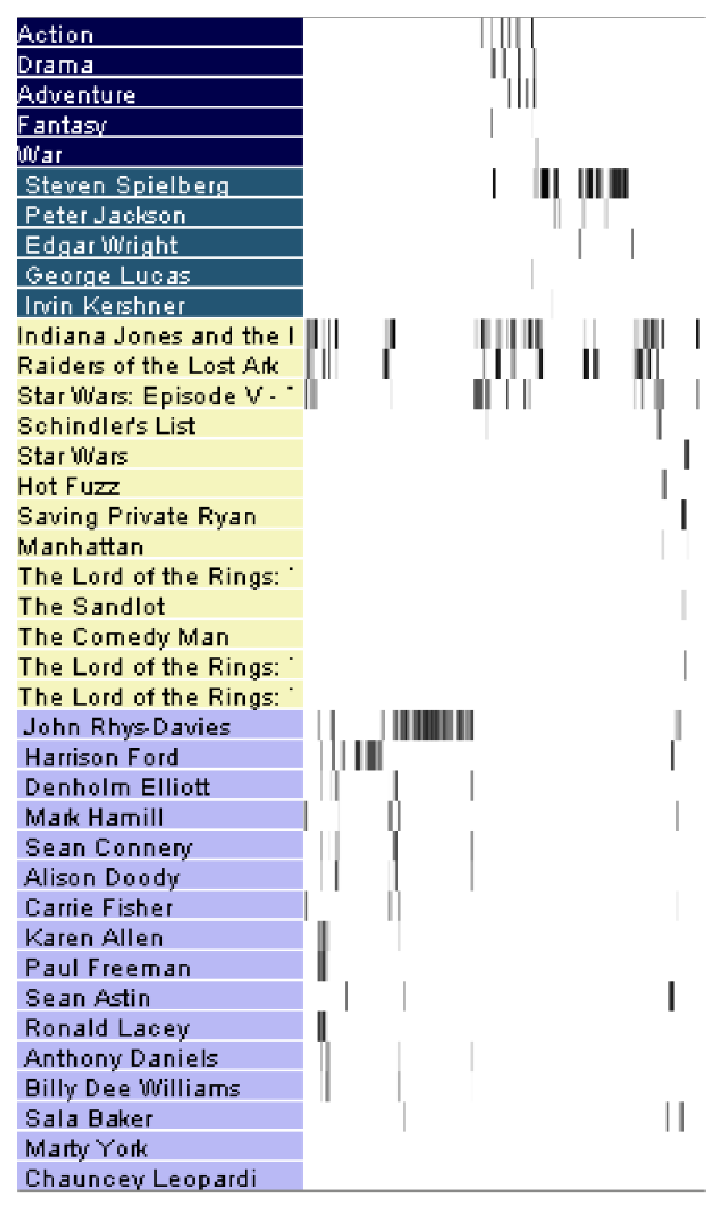
\includegraphics[width=\linewidth]{images/heatmap.eps }
  \caption{Visualization of DOI streaming from multiple users concurrently. For each user, ten most viewed objects in the last $90$ seconds are listed vertically, ordered and scaled by the amount of interest the user showed in them. Time advances horizontally (most recent moment on the right), and color indicates the degree of interest in an object at every $1$ second interval.}
	\label{fig:heatmap}
\end{figure}


